\section{Селективное лазерное спекание}


\subsection{Технология}

Описание технологии 3D-печати по методу СЛС взято из \cite{sls-material, ageing}.

\begin{figure}[ht]
    \centering
    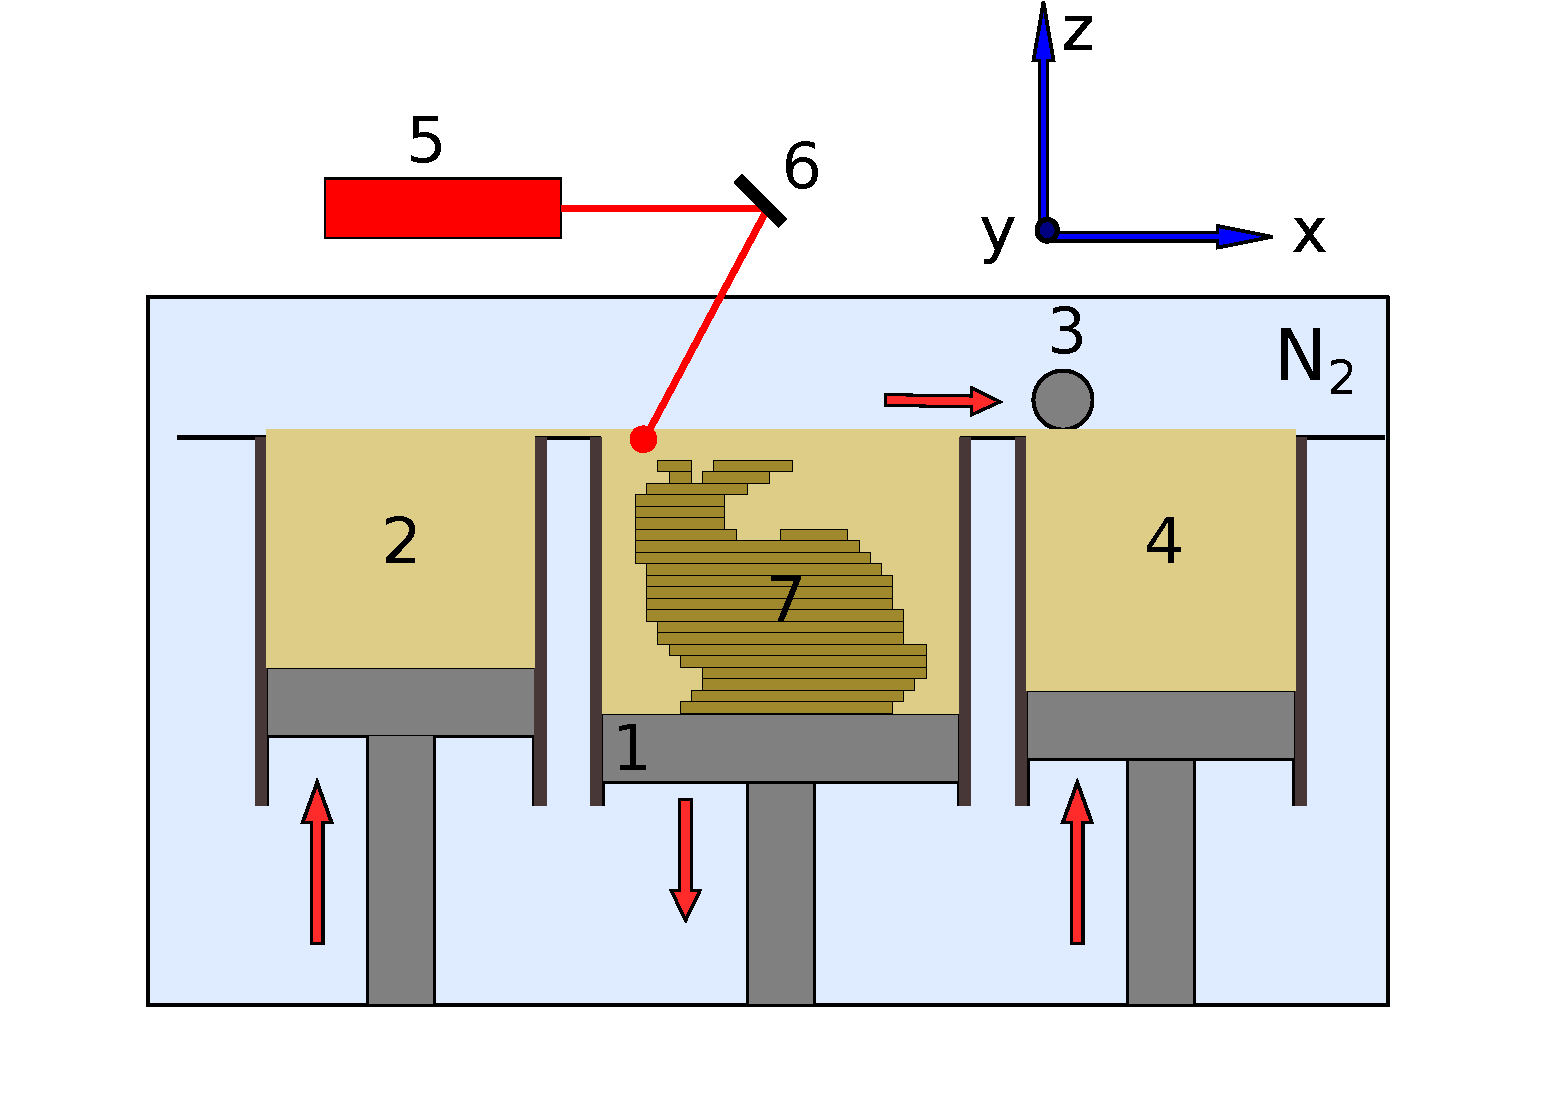
\includegraphics[width=\linewidth]{fig/sls-2d.pdf}
    \caption{Схематическое изображение работы СЛС-принтера.}
    \label{fig:printer}
\end{figure}


В процессе СЛС лазер послойно сканирует подложку с порошком и спекает частицы порошка, таким образом формируя заданную объемную структуру, как продемонстрированно на рис. \ref{fig:printer}. 

Порошок подается на сборочную платформу(1) из контейнера (2) и распределяется по ней тонким слоем с помощью ролика (3), двигающегося по оси $x$. Типичная толщина слоя составляет от 50 до 200 мкм. Остатки порошка собираются в контейнер (4).
CO$_2$-лазер(5), снабженный соответсвующей оптической системой(6), сканирует слой по заданным координатам.
После сканирования каждого слоя, платформа сдвигается вниз по оси $z$ на глубину, равную толщине слоя. В процессе печати, так называемый колодец построения (7) "растет" снизу вверх. В объемном соотношении, он обычно состоит примерно на 90\% из неспеченного порошка, а изделие занимает только около 10\%. 
Как правило, перед спеканием порошок дополнительно прогревается.
На этом этапе неспеченный порошок и расплавленные части остаются в квази-изотермических условиях внутри одного слоя.
Температура при этом должна быть ниже температуры плавления, но выше температуры рекристаллизации, для предотвращения коробления материала в процессе печати.
Для предоствращения окисления полимера камера продувается азотом (с остаточным содержанием кислорода не более 2\%). По завершению печати, изделие вместе с оставшимся порошком сначала охлаждается в атмосфере азота в течение примерно 10 ч, а затем вне принтера до тех пор, пока температура не опустится ниже температуры стеклования.

Затем, изделие отделяется от неспеченного порошка. В целом, при высоте изделия до 60 см, характерной толщиной слоя 100 мкм и временем сплавления на слой от 10 до 40 с, процес производства может занимать многие часы и дни, в результате чего просихдит старение полимера. В связи с этим актуален синтез термостабильных материалов, как с точки зрения свойств конечного изделия, так и с точки зрения повторного использования неспеченного порошка.

\paragraph{Особенности}
Помимо общих особенностей, характерных для технологий аддитивного производства, таких как..., селективное лазерное спекание также имеет свои преимущества.
\begin{itemize}
    \item Хорошие характеристики изделий, сходные с традиционным производством.
    \item Остатки порошка можно использовать повторно
    \item Напечатанные части остаются в неиспользованном порошке, поэтому, в отличие от других методов 3D-печати, не требуют специальных опорных конструкций.
    \item Теоретически, возможна обработка методом СЛС любого вещества, которое можно перевести в порошкообразную форму и спечь при повышенной температуре\cite{vaganov}.
\end{itemize}

\subsection{Сращивание частиц порошка}
Консолидация частиц порошка под воздействием лазерного излучения на полимерный материал, расположенный на "сборочной платформе" как правило называют селективным лазерным спеканием (Selective laser sintering, SLS) или селективым лазерным cплавлением (Selective laser melting, SLM). Различие между этими двумя методами неопределенное и не охватывает все механизмы, по которым происходит сращивание порошка в трехмерное изделие.

Процессы спекания/спдавдения могут быть разбиты на следующие категории \cite{comp-review, consolidation}: твердотельное спекание, жидкофазное спекание/частичное плавление, полное плавление, и химическое связывание. Классификация схематически показана на рис.\ref{fig:binding}



Твердофазное спекание - процесс, который происзодит за счет диффузии при температурах между $T_{melt}/2$ и $T_{melt}$, где $T_{melt}$ -- температура плавления. В жидкофазном спекании, как правило, связующий материал  плавится,в то время как структурный материал остается твердым. В техниках полного плавления порошок плавится полностью, и показывает свойства, сравнимые со свойствами объемного материала. Полимерны материалы как правило используются в двух последних.



\begin{figure}[h]
    \centering
    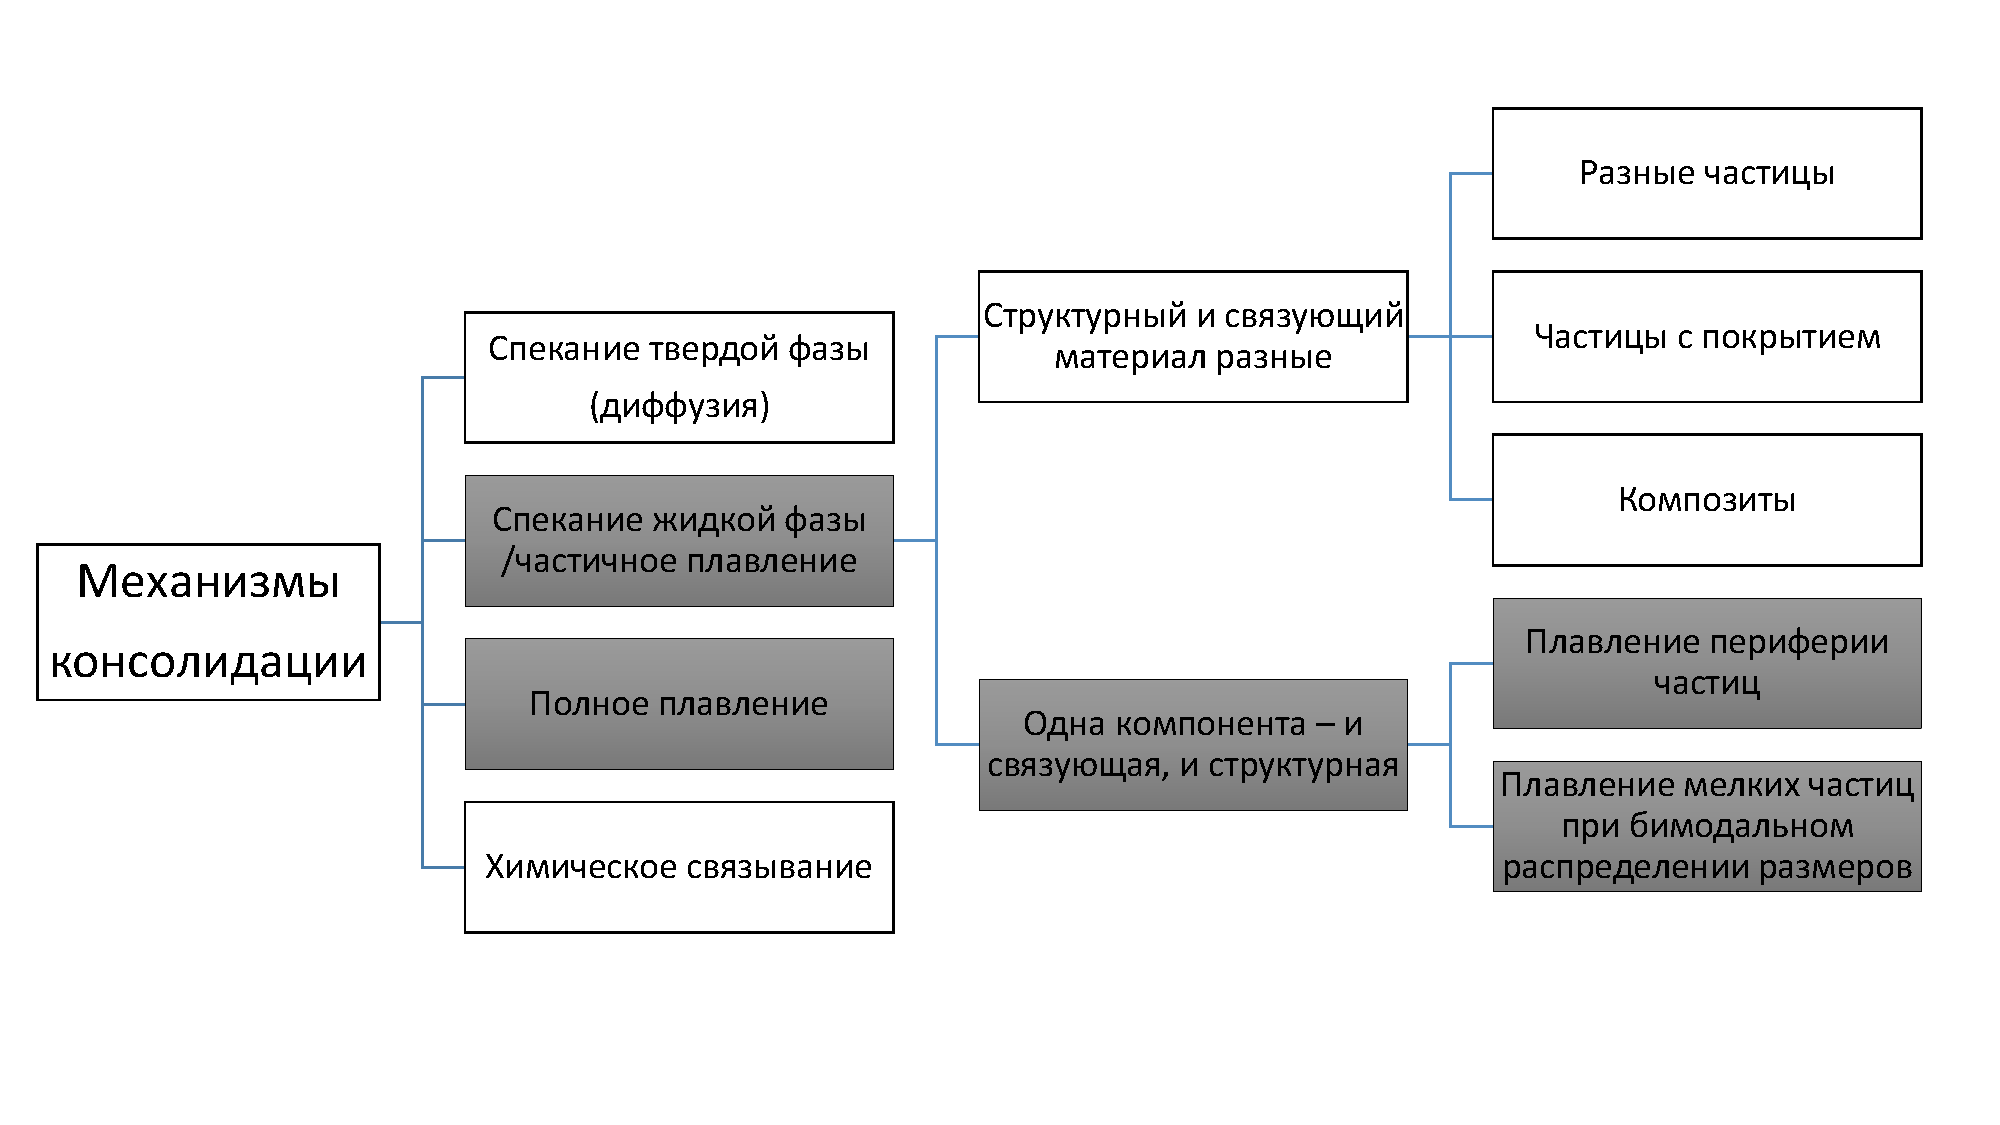
\includegraphics[width = \linewidth]{fig/mecha.pdf}
    \caption{Механизмы консолидации порошков при СЛС}
    \label{fig:binding}
\end{figure}

\section{Кристаллическая структура полимеров}

\subsection{Общие сведения}

	\begin{wrapfigure}{r}{0.5\textwidth} 
\vspace{-20pt}


  \begin{center}
    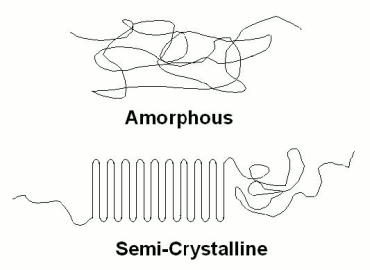
\includegraphics[width=0.4\textwidth]{fig/crystal-1.png}
    \caption{Полимерная цепь в аморфном и частично-кристаллическом состоянии}
    \label{fig:crystal-1}
  \end{center}
  \vspace{-20pt}
  \vspace{1pt}
\end{wrapfigure}


Поскольку кристаллические области в этих полимерах формируются из длинных цепей, их кристаллизация сложна и сильно чувствительа к маленьким изменениям в составе, добавкам, температуре и механическим воздействиям.\\
Кристаллическая структура полимеров менее идеальна чем кристаллы соединений с меньшей молекулярной массой. Как правило полимерные материалы находятся в метастабильном состоянии, то есть являются частично кристаллическими и частично аморфными. Только небольшая часть кристаллизуемых цепей оказывается включенной в кристаллические домены, а остальные отделяются к аморфным областям. Степеь кристалличности и характеристики кристаллических доменов являются самыми важными морфологическими характеристиками, которые определяют физические свойства такие как плотность, механическую прочность и  пригодность для обработки,  частичнокристаллического полимера.
Степень кристалличности типичного полимера варьируется в пределах от 10 до 80 \%. Это явно отличает  полимерны материалы от, например, металлов, которые, за исключением металлических стекол, почти всегда полностью кристалличны, или керамических материалов, которые или полностью кристалличны, или аморфны \cite{cryst1}.

Кристаллическая структура и степень кристалличости зависят от молекулярной структуры полимера, условий роста кристаллов, присутствия инородых частиц в решетке, температуры кристаллизации, скорости охлаждения и т.д.\\
Они могут быть оценены из рентгеновской дифракции, измерений плотности, термического анализа и и других методов.

\subsection{Кристаллиты}
Морфологии полимерных кристаллов можно условно поделить на ламеллярные и фибриллярные кристаллы. В процессе ламеллярной кристаллизации, направление роста перпендикулярно направлению цепи, возникает складываение цепочки.Во время фибриллярной кристаллизации, наплавление роста кристалла совпадает с направление цепи, и в решетке кристалла появляются сильно вытянутые  цепи. Такие материалы имеют высокие механические свойства. Кристаллизация существенно меняет физические и механические свойства полимерных систем. \\


\subsection{Частичная кристалличность}

Свойства частичнокристаллических полимеров можно понять, по большей части, используя простую двухфазную модель, которая предполагает, что две фазы, кристаллическая и аморфная, легко различимы. Если интенсивный параметр  $\phi$ (например, удельный объем) кристаллической и аморфной фазы , $\phi_c$ и $\phi_c$, соответственно, может быть измерен, и мы предполагаем, что вклады двух фаз являются аддитивными, тогда
\[ 
\phi = \phi_c x + \phi_a(1-x),
\]
где $x$  -- доля кристаллической фазы, чаще всего массовая, хотя это в некоторой степени зависит от метода измерения \cite{cryst3}.
	
Модель двух фаз, которой мы пользуемся, разумеется, является лишь приближением, поскольку в материале может оказаться сколько угодно типов структур: от огромных идеальных монокристаллов до чисто аморфных областей, с ближним порядком по типу жидкости.
Из-за ограничений, которые накладывают на структуру длинные полимерные цепи, в кристаллической решетке всегда присутствуют дефекты, а полимерные кристаллиты маленькие и беспорядочно расположенные. В свою очередь, аморфные домены обладают некоторой степенью позиционной и ориентационной кореллированности.
Нельзя всегда сделать четкого различия между сигналами кристаллической и аморфной фазы. Тем не менее, модель двух фаз с прибилженной аморфной и кристаллической фазой, иногда с добавлением еще одной упорядоченной фазы используется чаще всего.